\subsection{Instruction Working Set Signature}

An instruction working set (IWS)~\cite{Dhodapkar:2002:MMH} is the set of instructions touched over a fixed interval of time. The relative working set distance between intervals $i$ and $i-1$ is defined as 

\begin{center}
$\delta_{i,i-1} = \frac{||W_i \bigcup W_{i-1}||-||W_i \bigcap W_{i-1}||}{||W_i \bigcup W_{i-1}||}$
\end{center}
where $W_i$ is the working set for interval $i$.
 
A working set signature is a lossy-compressed representation of a working set. The program counter is sampled over a fixed interval of instructions. A hashing function is applied to the sample to set a bit in an $n$-bit vector, which represents the signature (See Figure~\ref{fig:signature}). Phase changes are detected by computing the relative signature distance between intervals and comparing the distance against some pre-determined threshold. The hardware complexity of this technique is dependent on the working set size.

\begin{figure}[htbp]
  \begin{center}
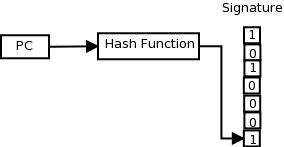
\includegraphics[width=0.60\columnwidth]{figs/workingsetsignature}
  \end{center}
  \caption{Generating the working set signature.}
  \label{fig:signature}
\end{figure}
